%%%%%%%%%%%%%%%%%%%%%%%%%%%%%%%%%%%%%%%%%%%%%%%%%%%
%% P3: Phenomenology of Particle Physics                         
%%
%% Author:  André Rubbia                   		 
%%
%% Figure 2.1 A comparison of the experimental black-body data with the Rayleigh--Jeans and the Planck theories.
%%
%% This work is licensed under the Creative Commons Attribution 4.0 International License. 
%% To view a copy of this license, visit http://creativecommons.org/licenses/by/4.0/ or 
%% send a letter to Creative Commons, PO Box 1866, Mountain View, CA 94042, USA.
%%
%%%%%%%%%%%%%%%%%%%%%%%%%%%%%%%%%%%%%%%%%%%%%%%%%%%

\documentclass[a4paper,10pt]{article}

\usepackage[T1]{fontenc}
\usepackage[utf8]{inputenc}
\usepackage{lmodern}
\usepackage[labelfont=bf]{caption}
\usepackage{upgreek}

\usepackage{tikz}
\usepackage{pgfplots}
\pgfplotsset{compat=1.17}
\usepgfplotslibrary{ternary}
\usepgfplotslibrary{fillbetween}
\usepgfplotslibrary{external}

\def\d{\mathrm{d}}

\begin{document}

%%%%%%%%%%%%%%%   FIGURE  %%%%%%%%%%%%%%%%%%%%%%%%%%%%%%
\begin{figure}[htb]
\begin{center}
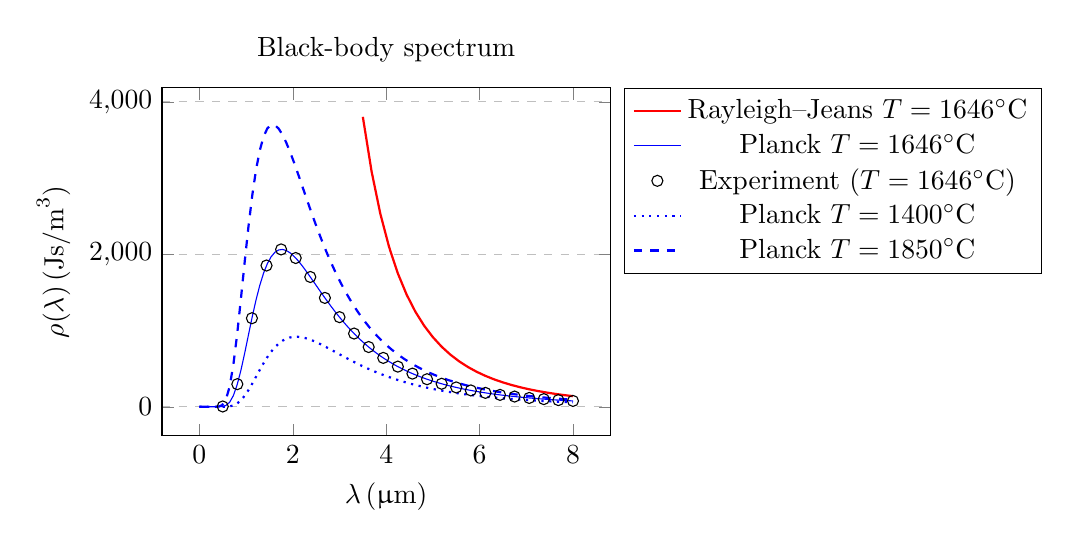
\begin{tikzpicture}[scale=1]
\begin{axis}[
    width=0.6\textwidth, height=6cm,
    title={Black-body spectrum},
    xlabel={$\lambda\, (\upmu\mathrm{m})$},
    ylabel={$\rho(\lambda)\, (\mathrm{Js/m}^3)$},
    legend pos=outer north east,
    ymajorgrids=true,
    grid style=dashed,
]
 \addplot[domain=3.5:8,thick,
    color=red]
    {8*3.14*1.38e-23*1646/((x/1e6)^4};
 \addplot[domain=0:8,samples=100,
    color=blue]
    {8*3.14*6.625e-34*3e8/(x/1e6)^5*(1/(exp(6.625e-34*3e8/((x/1e6)*1.38e-23*1646))-1))};
\addplot[domain=0.5:8,samples=25,mark=o,only marks,
    color=black]
   {8*3.14*6.625e-34*3e8/(x/1e6)^5*(1/(exp(6.625e-34*3e8/((x/1e6)*1.38e-23*1646))-1))};
 \addplot[domain=0:8,samples=100,dotted,thick,
    color=blue]
    {8*3.14*6.625e-34*3e8/(x/1e6)^5*(1/(exp(6.625e-34*3e8/((x/1e6)*1.38e-23*1400))-1))};
 \addplot[domain=0:8,samples=100,dashed,thick,
    color=blue]
    {8*3.14*6.625e-34*3e8/(x/1e6)^5*(1/(exp(6.625e-34*3e8/((x/1e6)*1.38e-23*1850))-1))};
     \legend{Rayleigh--Jeans $T=1646^\circ$C,Planck $T=1646^\circ$C,Experiment ($T=1646^\circ$C),
     Planck $T=1400^\circ$C,Planck $T=1850^\circ$C}
\end{axis}
\end{tikzpicture}
\caption{A comparison of the experimental black-body data with the Rayleigh--Jeans and the Planck theories.
The experimental points illustrate data at a temperature $T=1646^\circ$C.}
\end{center}
\end{figure}
%%%%%%%%%%%%%%%   FIGURE  %%%%%%%%%%%%%%%%%%%%%%%%%%%%%%
%

\end{document}
